\begin{savequote}[75mm]
vulputate egestas, eros pede varius leo.  \qauthor{Quoteauthor Lastname}
\end{savequote}

\chapter{Wprowadzenie}
Teoretyczne rozważania dotyczące pochodzenia planet mają długą historię
sięgającą przynajmniej XVIII wieku, kiedy to Immanuel Kant wysunął \dq{}Hipotezę
mgławicową\dq{}. Już wtedy unikalność Układu Słonecznego stanowiła przedmiot
debaty. Dopiero na początku XX wieku pogląd, iż układy planetarne są czymś
powszechnym we Wszechświecie, został zaakceptowany przez środowisko naukowe, a w
roku 1992 została odkryta pierwsza, pozasłoneczna planeta orbitująca pulsar PSR
1257+12 b~\cite{1992Natur.355..145W}.

W połowie XVIII wieku, filozof francuski Immanuel Kant zasugerował, iż rozmyte
o\-biek\-ty obserwowane przez niego przez teleskop mogą być wyspowymi
Wszechświatami takimi jak nasz, bądź obłokami materii w których formują się
gwiazdy i planety~\cite{ImmanuelKant.etal:2008}.

\begin{figure}[!ht]
\centering
%\includegraphics[width=0.8\textwidth]{figures/laplace.png}
\caption{Model mgławicy Laplace'a: (a) rotująca mgławica; (b) kolapsująca
mgławica ulega spłaszczeniu wzdłuż osi rotacji; (c) soczewkowaty kształt
mgławicy; (d) pierścienie materii pozostawione przez zapadający się obiekt
centralny; (e) zagęszczenia na poszczególnych pierścieniach kolapsują tworząc
planety. (Obrazek z pracy Woolfson, 1993)} 
\label{fig:laplace}
\end{figure}

\section{Paradygmat formowania się planet}
Formowanie się planet jest nierozerwalnie związane z narodzinami gwiazd, które
biorą swój początek w gęstych pyłowo--gazowych obłokach materii. Zanurzone w
gorącym ośrodku międzygwiazdowym, początkowo w stanie równowagi termodynamicznej
z otaczającym je gazem, obłoki takie często występują w
ogromnych kompleksach i obserwowane są jako ciemne mgławice molekularne. {\bf
(see Tielens 2005 for a review on a phases of the ISM)} Procesy zachodządze w
samych obłokach, tj. turbulencja, samograwitacja, lub w ośrodku zewnętrznym tj.
wybuchy supernowych mogą powodować wzrost gęstości poszczególnych zagęszczęń w
obłoku. W momencie w którym obszar gęstej materii przekroczy  masę krytyczną,
nazywaną masą Jeansa $M_J$, grawitacja przeważa i chmura zaczyna się zapadać
(rysunek 1a). Masa Jeansa zależy od temperatury kinetycznej ośrodka $T$ oraz
jego gęstości $\rho$ \begin{equation} M_J \sim \left( \frac{k_B T}{G} \right)
^\frac{3}{2} {\rho}^{-\frac{1}{2}}, \end{equation} gdzie $k_B$ jest stałą
Boltzmanna a $G$ jest stałą grawitacji. Dla typowych warunków panujących
wewnątrz obłoków materii międzygwiazdowej, masa Jeansa przyjmuje wartość
\begin{equation}
 M_J \approx 2.9 M_{\odot} \left(\frac{T}{\textrm{10 K}}\right)^{1.5} 
 \left(\frac{n}{10^4\thinspace \textrm{cm}^{-3}}\right)^{-0.5},
\end{equation}
gdzie $n = \rho_g / \mu m_{\textrm{H}}$ jest koncentracją cząstek materii.
Kolaps obłoku następuje w tzw. skali czasowej spadku swobodnego
\begin{equation}
   t_{\textrm{ff}} \sim \frac{1}{\sqrt{G\rho}} \sim 10^5\thinspace\textrm{yr}
   \left(\frac{n}{10^4\thinspace \textrm{cm}^{-3}}\right)^{-0.5},
\end{equation}
co z punktu widzenia całkowitego czasu potrzebnego do uformowania się planet
jest czasem relatywnie krótkim. Podczas kolapsu energia
grawitacyjna zapadającego się obłoku jest przekształcana w energię termiczną.  W
wypadku braku efektywnego mechanizmu chłodzenia się gazu, temperatura wewnątrz
obłoku wzrasta (a wraz z nią masa Jeansa) zatrzymując dalszy kolaps
grawitacyjny. Obserwacyjna klasyfikacja formujacego się układu protoplanetarnego
określa obiekty na tym etapie mianem obiektów \emph{klasy 0}~\cite{andre} (rysunek 1b).
Ich obserwowana temperatura jest stosunkowo niska $(T \lesssim
30\thinspace\textrm{K})$. Obiekty tej klasy charakteryzują się maksimum w
rozkładzie energii promieniowania wypadającym w dalekiej podczerwieni, bez
wykrywalnej nadwyżki w bliskiej podczerwieni.
Kolejnym krokiem ewolucji zapdającego się obłoku jest rozpalenie reakcji
termojądrowych w centrum. Pole promieniowania pochodzące od protogwiazdy
podgrzewa opadająca materię i formujący się dysk do temperatury $T \sim
100\thinspace\textrm{K}$ tworząc obiekt \emph{klasy I} (rysunek 1c).  Część
akreująca z dysku materii w pewnym momencie zostaje uniesiona z gwiazdy w
postaci silnego wypływu, który wybija dziurę w otoczce progwiazdowej. Wydarzenie
to może być bardzo gwałtowne i znacznie wpłynąć na tempo akrecji i co za tym
idzie jasność obiektu. Gwałtowny wybuch zwyczajowo nazywa się \emph{rozbłyskiem
FU--Orionis}.
W obiektach \emph{klasy I} maksimum w rozkładzie energii promieniowania przesuwa
się w kierunku bliskiej podczerwieni, praktycznie wypłaszczając widmo.  \par Po
około $10^5$ lat, większość otoczki zostaje odrzucona przez wiatr, a dysk
protogwiazdowy zostaje zredukowany do kilku procent masy gwiazdy macierzystej.
Osiągana jest bardziej stabilna konfiguracja, tzw. faza \emph{T-Tauri} dla
gwiazd o masach mniejszych niż $2\thinspace\Msun$, badź faca \emph{Herbig Ae/Be}
dla gwiazd masywniejszych. Dla obiektów tej klasy (\emph{klasa II} rysunek 1d)
znacznie spada nadwyżka w podczerwieni. Okres ten trwa od $10^5$ do $10^6$ lat.

% Pozniej
%Na tym etapie musi nastąpić formacja planetezymali i gazowych olbrzymów,
%ponieważ po jej zakończeniu dysk protoplanetarny zanika.  Pozostaje gwiazda
%zbliżająca się do ciągu głównego, nie wykazująca już żadnej nadwyżki w
%podczerwieni --- obiekt \emph{klasy III} (rysunek 1e).

\begin{figure}[p]
\centering 
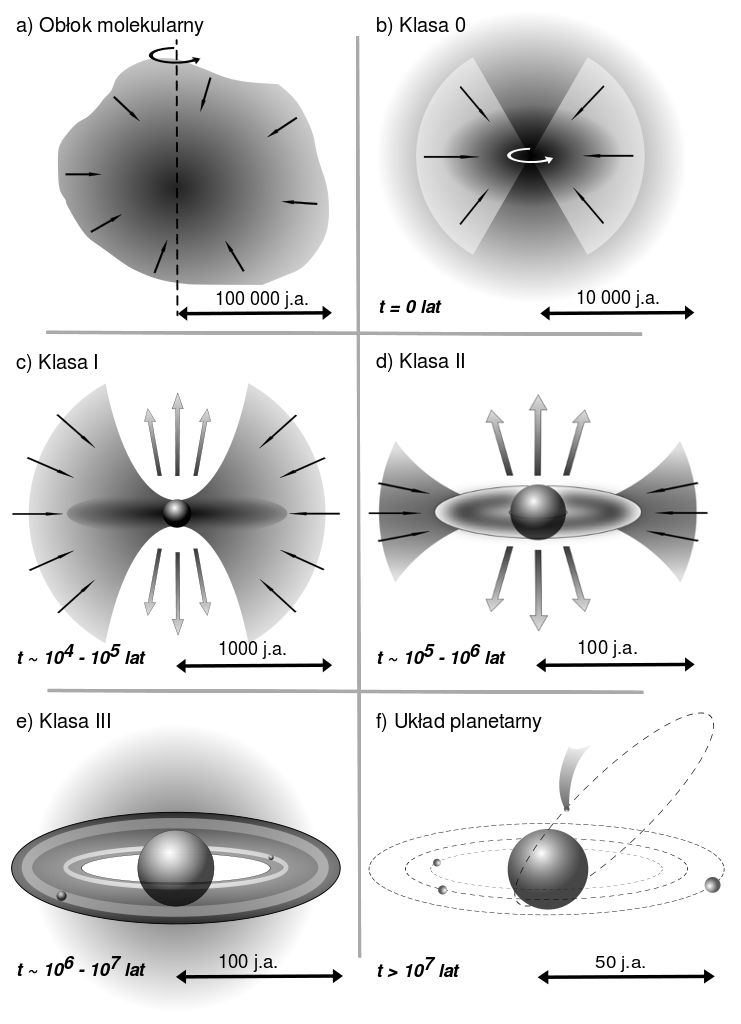
\includegraphics[width=0.9\textwidth]{figures/planetformation.png}
\caption{Ilustracja przedstawia kolejne fazy formowania się małomasywnej gwiazdy
wraz z systemem planetarnym: a) kolaps grawitacyjny gęstego obłoku; b)
oddziaływanie centralnego pola grawitacyjnego oraz siły odśrodkowej powoduje
opadanie materii i formowanie się dysku; c) faza FU Orionis: silna akrecja w
dysku oraz wypływ materii w okolicach osi obrotu; d) faza T Tauri: zmniejsza się
tempo akrecji oraz wypływu materii, rozpoczyna się proces formowania planet; e)
zanika składowa gazowa, planety otwierają przerwy w dysku, następuje również ich
migracja; f) cały gaz oraz mniejsze ciała zostają pochłonięte przez planety lub
usunięte z dysku, układ planetarny przyjmuje ostateczny kształt.}
\label{fig:planet} \end{figure}

%\section{Faza T Tauri}

Podczas tej fazy większość energii wyświecanej przez gwiazdę pochodzi ciągle z
energii grawitacyjnej traconej podczas kontrakcji. Ewolucja zachodzi w tzw.
skali czasowej Kelvina--Helmholtza 

\begin{equation} 
   t_{KH} \sim  \frac{G{M_{\star}}^2}{R_{\star}L_{\star}} = 3\cdot
   10^7\thinspace\textrm{yr} 
   \left(\frac{M_\star}{M_\odot}\right)^{2}
   \left(\frac{L_\star}{L_\odot}\right)^{-1}
   \left(\frac{R_\star}{R_\odot}\right)^{-1}
\end{equation}

gdzie $M_{\star}$, $R_{\star}$, $L_{\star}$ są odpowiednio masą, promieniem i
dzielnością promieniowania gwiazdy. Formująca się gwiazda powoli przesuwa się na
diagramie Hertzsprunga--Russela w kierunku ciągu głównego wieku
zerowego~\cite{palla}.  Dla gwiazd o masie Słońca ewolucja ta będzie przebiegała
po tzw. ścieżce Hayashiego, na której obiekty pozostają całkowicie konwektywne,
podczas gdy gwiazdy bardziej masywne utworzą promieniste jądra i przesuną się
w stronę wyższych temperatur. W tym czasie otaczający gwiazdę dysk traci
gaz na skutek fotoewaporacji i wiatru gwiazdowego. Zarówno obserwacje gwiazd
T-Tauri jak i rozważania teoretyczne~\cite{alexanderpassuci2013} {\bf and ref
therein} szacują że proces utraty gazu z dysku trwa od jednego do kilku Myr.
Stanowi to niewątpliwie limit na wytworzenie się gazowych olbrzymów, tj. w dysku
protoplanetarnym muszą wcześniej wytworzyć się obiekty zdolne akreaować wodór.

\par Po dyspersji dysku gazowego gwiazda powoli traci również nadwyżkę w
podczerwieni. Sugeruje to ubytek materiału pyłowego z układu

\section{Ważne pojęcia}
Od gazowego dysku, stopniowe przejście do efektów pyłu

\subsection{Struktura dysku protoplanetarnego}
Proces kolapsu grawitacyjnego, sferycznego obłoku materii międzygwiazdowej nie
wpływa na jego całkowity moment pędu. Przy założeniu, że obłok rotuje, nawet
bardzo wolno, to materia nie opada bezpośrednio na obiekt
centralny, lecz formuje dysk w płaszczyźnie prostopadłej do wektora całkowitego
momentu pędu. Aby określić przybliżone warunki fizyczne w formującym się dysku
możemy posłużyć się równaniami hydrodynamiki:

\begin{gather}
\partial_t \rho_g + \nabla\cdot\left(\rho_g\mathbf{u}\right) = 0,\\
\partial_t \mathbf{u} + \left(\mathbf{u}\cdot\nabla\right)\mathbf{u} = 
-\nabla\Phi + -\frac{1}{\rho_g} \nabla P 
\end{gather}

gdzie $\rho_g$ jest gęstością gazu, $P$ ciśnieniem, 
związanych z tarciem, a $\Phi$ potecjałem grawitacyjnym. Jeżeli ponadto
założymy, że dysk:

\begin{enumerate}
   \item jest izotermiczny to $P = c_s^2 \rho_g \implies -\frac{1}{\rho_g}\nabla
      P = -c_s^2\nabla\ln\rho_g$, gdzie $c_s = \sqrt{\frac{k_{\textrm{B}} T}{\mu
      m_{\textrm{H}}}}$ jest izotermiczną prędkością dźwięku.
   \item jest stacjonarny i znajduję się w równowadzę hydrostatycznej w kierunku
      $z$ to wertykalne przyspieszenie grawitacyjne $\partial_z \Phi = g_z =
      (GM_\star/r^2) z/r = \Omega^2 z$, gdzie $M_\star$ to masa gwiazdy
      macierzystej, $\Omega$ orbitalna częstość keplerowska, $G$ stała
      grawitacji Newtona, jest równoważone przez siłę wynikająca z gradientu
      ciśnienia gazu $\partial_z P / \rho_g$
\end{enumerate}

Łącząc powyższe założenia otrzymujemy rozkład gęstości gazu

\begin{equation}
   \rho_g(z) = \frac{\Sigma_G}{H\sqrt{2\pi}} \exp \left[
   \frac{1}{2}\left(\frac{z}{H}\right)^2 \right],
\end{equation}

gdzie $\Sigma_g = \int \rho_g(z) dz$ jest gęstością powierzchniową, a
$H=\frac{c_s}{\Omega}$ to charakterystyczna skala grubości dysku.

%\par Zakładając w pierwszym przybliżeniu że dysk jest optycznie gruby, t.j.
%absorbuję całkowicie promieniowanie pochodzące od gwiazdy i następnie reemituje
%je jako ciało doskonale czarne, można pokazać~\cite{armitage07} że $T \propto
%r^{-3/4}$ i co za tym idzie $c_s \propto r^{-3/8}$. Dokładniejsze szacunki,
%które lepiej oddają obserwowane dystrucje spektralne energii, można znaleźć w
%pracach~\cite{KenyonHART87, ChaingGold97} {\bf patrz armitage}.
%{\bf Tu raczej trzeba przedstawić tę wersję z której wynika $T \propto
%r^{-1/2}$}
%
\par W modelu stacjonarnym w kierunku radialnym grawitacja i siła wynikająca z
gradientu ciśnienia jest równoważona poprzez siłę odśrodkową
\begin{equation}\label{eq:radial_balance}
\frac{u_\phi^2}{r} = \frac{GM_\star}{r^2} +
  \frac{1}{\rho_g}\frac{\textrm{d}P}{\textrm{dr}},
\end{equation}
gdzie $u_\phi$ jest prędkością orbitalną gazu. Wpływ gradientu ciśnienia na
globalną dynamikę jest znikomy (rzędu $O(H/r)^2$), dlatego dla cienkich dysków
$(H/r \ll 1)$ z dobrym przybliżeniem można przyjąć, że właściwy moment pędu dla
gazu jest równy momentowi pędu wynikającemu z ruchu keplerowskiego. Z równania
\mref{eq:radial_balance} wynika zatem, że moment pędu jest rosnącą funkcją
promienia:
\begin{equation}\label{eq:angmom}
l = r^2\Omega = \sqrt{GM_\star r}.
\end{equation}
Z równania \mref{eq:angmom} wypływa niezwykle ważny fakt: aby materiał z dysku
mógł być akreaowany przez gwiazdę macierzystą, w układzie musi działać mechanizm
powodujący utratę bądź chociaż redystrybucję momentu pędu.
\subsection{Niestabilność magnetorotacyjna}


\subsection{Niestabilność grawitacyjna}
\subsection{Oddziaływanie pomiędzy gazem, a pyłem}
\subsection{Radialny dryf pyłu}
\subsection{Sedymentacja i pułapkowanie pyłu (KHI)}
\subsection{Koagulacja i wzrost rozmiarów}
W fazie T Tauri następuje koagulacja ziaren pyłu. Z perspektywy obserwatorów
jest ona równoważna usuwaniu drobnego pyłu z dysku a, co za tym idzie, spadkowi
nadwyżki promieniowania w zakresie podczerwonym. Dzięki pracom obserwacyjnym
wiemy, że zanik tej nadwyżki dla długości fal charakterystycznych dla
wewnętrznych obszarów dysków (wyższa temperatura) zajmuje ok. $10^6$ lat
\cite{hillenbrand}, natomiast zanik chłodnej składowej pyłowej następuje w
skalach czasowych ok. $2$ rzędy wielkości większych \cite{carpenter}.

Skala czasowa $t$ koagulacji pyłu, wynikająca z analizy drogi swobodnej cząstek,
wyraża się poprzez \begin{equation}\label{coag} t \sim \frac{a}{\Delta
v}\frac{\rho_p}{\rho_d}, \end{equation} gdzie $a$ jest promieniem cząstki pyłu
(przy założeniu jednorodnego rozkładu rozmiarów cząstek), $\Delta v$ jest
średnią prędkością względna cząstek, $\rho_p$ jest gęstością materiału
budującego cząstki natomiast $\rho_d$ jest gęstością ośrodka pyłowego w dysku.
Przyjmując typowe wartości $a \approx 1$ $\mu$m, $\Delta v \approx 1$ cm/s,
$\rho_p \approx 2$ g/cm$^3$,  $\rho_d \approx 10^{-12}$ g/cm$^3$ otrzymujemy $t$
rzędu kilku lat. Teoretycznie cząstki mogłyby więc szybko zwiększyć rozmiary od
mikrometrowych do metrowych i większych. Na przeszkodzie stoją jednak własności
agregatów pyłowych związane z ich budową wewnętrzną oraz to, że prędkości
względne cząstek rosną wraz z ich rozmiarami. Po osiągnięciu pewnych rozmiarów
cząstki stają się zbyt kruche a ich prędkości względne zbyt duże, aby mógł
zachodzić dalszy wzrost.

%\section{Metrowa bariera wzrostu}
Cząstki pyłu sklejają się dzięki oddziaływaniom międzycząsteczkowym, które są
szczególnie wydajne w przypadku małych cząstek i dużego ich zagęszczenia. Takie
warunki występują w dysku protoplanetarnym. Wraz ze wzrostem cząstek proces
zlepiania zachodzi coraz wolniej. Koagulacja faworyzuje małe cząstki, które mają
większy stosunek powierzchni do masy. Prędkości względne cząstek w ogólności
rosną, gdy cząstki osiągną masę pozwalającą na odsprzęgnięcie się od gazu, co
również utrudnia dalszy wzrost. Nawet bez silnych ruchów turbulentnych gazu, w
odległości $1$ j.a. od gwiazdy metrowe cząstki osiągają prędkości względne rzędu
$10$ m/s. Zderzenia przy tak wysokich prędkościach względnych prowadzą do
fragmentacji cząstek. Zjawisko to jest w literaturze nazywane metrową barierą
wzrostu (ang. {\it meter-size barrier}) \cite{ormel}. Co więcej, oddziaływanie
cząstek z gazem powoduje utratę momentu pędu i szybki dryf radialny cząstek w
kierunku gwiazdy. Stanowi to~kolejne ograniczenie czasowe ($\sim 10^2$ lat) dla
procesu formowania się planet.

Aby planety mogły powstać, metrowa bariera wzrostu musi być pokonana w
stosunkowo krótkiej skali czasowej. Nie jest jasne, czy zwykłe mechanizmy
sklejania są wystarczające aby otrzymać cząstki o rozmiarach rzędu kilometrów,
dla których dopiero zaczynają odgrywać rolę oddziaływania grawitacyjne. Istnieje
alternatywna teoria, w której metrowa bariera wzrostu jest pokonywana dzięki
wystąpieniu w pyle niestabilności grawitacyjnej. Niestabilność ta wymaga jednak
wysokich koncentracji cząstek o stosunkowo niskich prędkościach względnych.
Możliwość występowania niestabilności grawitacyjnej w pyłowej składowej dysków
protoplanetarnych jest wciąż przedmiotem naukowej dyskusji \cite{gi1,gi2}.

\subsection{Niestabilność strumieniowa}
\section{Cel pracy}
Głównym celem pracy jest zbadanie niestabilności strumieniowej w bardziej
realistycznym przyblizeniu radialnie rozciągłego dysku.

\newthought{Skąd wzięły się planety?} Pytanie które nurtuję ludzkość od
zamierzchłych czasów 

\section{Luźne myśli}

Formowanie się planet jest złożonym procesem, który wymaga wzrostu rozmiaru
mikrometrowych ziaren pyłu o wiele rzędów wielkości. Pomimo tego, że najmniejsze
drobiny pyłu są silnie sprzężone z gazem, mogą one dryfować zarówno w kierunku
radialnym jak oraz wertykalnym i podlegać wzajemnym zderzeniom. Przy odpowiednio
niskiej prędkości względnej, taka kolizja może prowadzić do tworzenia coraz to
większych aglomeratów cząstek~\citep{BW08}. Z drugiej strony, ciała o rozmiarach
setek czy tysięcy metrów są na tyle duże, iż opór aerodynamiczny stawiany na nie
przez gaz jest całkowicie zaniedbywalne, zaś dominująca dynamicznie siłą są
wzajemne oddziaływania grawitacyjne~\citep{KKI06}.

\par Nierozwiązaną dotąd zagadką współczesnej astrofizyki jest pośredni etap
wzrostu centymetrowych ziaren pyłu do kilometrowych głazów stanowiących budulec
planet. Istnieje szereg procesów, które przeciwdziałają możliwemu wzrostowi
rozmiaru ziaren pyłu lub nakładają silne więzy czasowe na formację systemów
planetarnych. Najsilniejszym ograniczeniem jest szybki radialny dryf dla ziaren
pyłu luźno związanych z gazem, tj. takich dla których charakterystyczna skala
czasowa dla tarcia aerodynamicznego jest porównywalna z ich okresem
orbitalnym~\citep{W77}. Ponadto typowe prędkości drobiny pyłu o rozmiarach od
$1\textrm{ cm}$ do $1\textrm{ m}$ zawierają się w przedziale $1\div10\textrm{ m
s}^{-1}$, co sprawia że najbardziej prawdopodobnym rezultatem zderzenia jest
fragmentacja bądź odbicie~\citep{Z10}.

\par Jednym z możliwych scenariuszy formowania się planet jest szybki wzrost
gęstości pyłu na skutek sedymentacji ziaren, którą wymusza pionowa składowa
grawitacji pochodzącej od gwiazdy macierzystej. Po przekroczeniu wartości
krytycznej gęsta warstwa pyłu rozpada się pod własnym ciężarem~\citep{GW73}.
Należy jednak mieć na uwadzę, że sam proces sedymentacji może prowadzić do
wzbudzenia się niestabilności Kelvina-Helmholza~\cite{JHK06}, a to przeciwdziała
tworzeniu się cienkiej i ciężkiej warstwy pyłu w płaszczyźnie dysku. Ostatnie
badania pokazują że odpowiednio masywne i metaliczne dyski są nie wrażliwe na
ten proces~\citep{L10}.

{\bf więcej o niestabilnościach powodujących turbulencje}

\par Zdecydowaną wadę powyższej hipotezy jest całkowite zaniedbanie globalnej
turbulencji występującej w dyskach okołogwiazdowych, będącej jedynym
mechanizmem zdolnym do wyjaśnienia obserwowanych temp akrecji materii na
formujące się gwiazdy w ramach tzw. teorii $\alpha$-dysków~\citep{SS73}.
Obecnie za dominujący proces odpowiedzialny za turbulencję uważa się niestabilność
magnetorotacyjna~\citep{BH98}. Dopuszcza ona obecność w dysku obszarów pozbawionych
turbulencji np. w miejscach o niewystarczającym stopniu jonizacji gazu, jednakże
istnieje szereg innych zjawisk które mieszają płyn~\citep{LP10}.  {\bf Tu by się
pewnie przydało opisać}

\par Pomimo tych niesprzyjających warunków istnieje proces który dominuje
ewolucję pyłu w momencie w którym stosunek koncetracji ziaren pyłu do gęstości
gazu zbliża się do jedności. Tym mechanizmem jest {\it niestabilność
strumieniowa} po raz pierwszy przedstawiona w pracy~\cite{YG05}. Okazuje się, że
połączenie komulowanie się pyłu w lokalnych maksimach w rozkładzie ciśnienia
gazu i wzjamne oddziaływanie pomiędzy tymi dwoma składnikami dysku, prowadzi do
znacznego wzrostu koncentracji ziaren pyłu~\citep{J11}. Nawet zaniedbując efekt
samograwitacji w trakcie ewolucji niestabilności strumieniowej lokalna gęstość
pyłu może zwiększyć się tysiąckrotnie~\cite{JY07}, co może prowadzić do
wytworzenia się grawitacyjnie związanych obiektów~\cite{J07}. Ostatnie badania
niestabilności strumieniowej skupiały się na różnych aspektach fizycznych które
mają wpływ na jej rozwój t.j.: uwzględnienie szerokiego spektrum rozmiaru
cząstek pyłu~\cite{BS10a}, wpływ globalnego gradientu ciśnienia w dysku
okołogwiazdowym~\cite{BS10b}, stratyfikacja dysku~\cite{T12}. Niemniej jednak
wszystkie publikacje naukowe były ograniczone do lokalnego przybliżenia dysku.


%%%%%%%%%%%%%%%%%%%%%%%%%%%%%%%%%%%%%%%%%%%%%%%%%%%%%%%%%%%%%%%%%%%%%%%%%%%%%%%%
% vim: tw=80 ts=3: 
